
%%%%%%%%%%%%%%%%%%%%%%% file typeinst.tex %%%%%%%%%%%%%%%%%%%%%%%%%
%
% This is the LaTeX source for the instructions to authors using
% the LaTeX document class 'llncs.cls' for contributions to
% the Lecture Notes in Computer Sciences series.
% http://www.springer.com/lncs       Springer Heidelberg 2006/05/04
%
% It may be used as a template for your own input - copy it
% to a new file with a new name and use it as the basis
% for your article.
%
% NB: the document class 'llncs' has its own and detailed documentation, see
% ftp://ftp.springer.de/data/pubftp/pub/tex/latex/llncs/latex2e/llncsdoc.pdf
%
%%%%%%%%%%%%%%%%%%%%%%%%%%%%%%%%%%%%%%%%%%%%%%%%%%%%%%%%%%%%%%%%%%%


\documentclass[runningheads,a4paper]{llncs}

\usepackage{amssymb}
\setcounter{tocdepth}{3}
\usepackage{graphicx}
\usepackage[hyphens]{url}
\usepackage{textcomp}
\usepackage{listings}
\lstset{
        basicstyle=\ttfamily\scriptsize,
        upquote=true,
        showspaces=false,
        showstringspaces=false,
        showtabs=false,
        tabsize=2,
        frame=none,
        breaklines,
        numbers=none,
        framexleftmargin=2mm,
        xleftmargin=2mm,
}

\usepackage{url}
\newcommand{\keywords}[1]{\par\addvspace\baselineskip
\noindent\keywordname\enspace\ignorespaces#1}

%% Define a new 'smallurl' style for the package that will use a smaller font.
\makeatletter
\def\url@smallurlstyle{%
  \@ifundefined{selectfont}{\def\UrlFont{\sf}}{\def\UrlFont{\scriptsize\ttfamily}}}
\makeatother
%% Now actually use the newly defined style.
\urlstyle{smallurl}
\newcommand{\nofootnote}[1]{~#1}

\begin{document}

\mainmatter  % start of an individual contribution

% first the title is needed
\title{A Tweet Consumer's Look At Twitter Through Linked Data Goggles Via Google Analytics}

% a short form should be given in case it is too long for the running head
\titlerunning{A Tweet Consumer's Look At Twitter Through Linked Data Goggles Via Google Analytics}

% the name(s) of the author(s) follow(s) next
%
% NB: Chinese authors should write their first names(s) in front of
% their surnames. This ensures that the names appear correctly in
% the running heads and the author index.
%
\author{Thomas Steiner \and Arnaud Brousseau}
% the affiliations are given next; don't give your e-mail address
% unless you accept that it will be published
\institute{Google Germany GmbH, ABC-Str. 19, 20354 Hamburg, Germany\\
\url{{tomac|arnaudb}@google.com}}

%
% NB: a more complex sample for affiliations and the mapping to the
% corresponding authors can be found in the file "llncs.dem"
% (search for the string "\mainmatter" where a contribution starts).
% "llncs.dem" accompanies the document class "llncs.cls".
%


\maketitle

\begin{abstract}

\end{abstract}

\section{Introduction}

\subsection{Google Chrome Extensions}
Google Chrome extensions\footnote{Google Chrome Extensions: \url{http://code.google.com/chrome/extensions/index.html}. Text adapted from the description to be found there.} are small software programs that can be installed to enrich the browsing experience with the Google Chrome browser. They are written using a combination of standard Web technologies, such as HTML, JavaScript, and CSS. Chrome extensions bundle all their files into a single file that gets usually (but not necessarily) distributed through the Chrome Web Store. There are several types of extensions, for this paper we focus on extensions based on so-called content scripts. Content scripts are JavaScript programs that run in the context of Web pages, similar to the Firefox Greasemonkey extension\footnote{Firefox Greasemonkey extension: \url{http://www.greasespot.net/}}. By using the standard Document Object Model (DOM), they can read or modify details of the Web pages a user visits. Examples of such modifications are, e.g., changing hyperlinks to remove potential @target="\_blank" attributes, or increasing the font size.

\subsection{Google Analytics}
 
\section{Twitter Swarm NLP Extension}
With our Twitter Swarm NLP extension\footnote{\url{https://chrome.google.com/webstore/detail/dpbphenfafkflfmdlanimlemacankjol}}, we inject JavaScript code via a content script into the Twitter.com homepage. The extension first checks if the user is logged in, and if so, retrieves the tweets of the logged-in user's timeline one-by-one, and performs NLP analysis via a remote NLP Web service on each of the tweets. The extracted entities are then displayed on the righthand-pane of the Twitter.com homepage, and sent to Google Analytics for further processing.

\subsection{Twitter Swarm NLP Web Service}
\subsection{Dealing With Extracted Entites On the Client Side}
\subsection{Dealing With Extracted Entites On the Google Analytics Side}

\begin{figure}[h!]
  \centering
  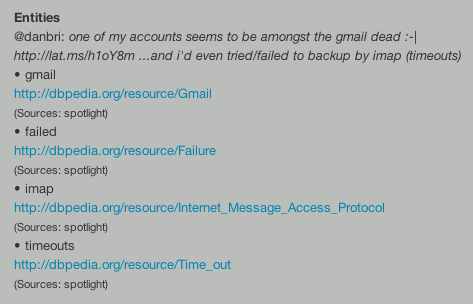
\includegraphics[width=0.6\linewidth]{danbri.png}
  \caption{Screenshot of the extracted entites of a particular tweet as displayed by the Twitter Swarm NLP Extension.}
  \label{fig:dataflow}
\end{figure}

\section{Related Work}
\subsection{Linked Open Social Signals (TWARQL)}
@ToDo Arnaud
\url{http://knoesis.wright.edu/library/download/paper-wi10-MPKS.pdf} \url{http://wiki.knoesis.org/index.php/Twarql}
\subsection{Twopular}
@ToDo Arnaud
\url{http://twopular.com/tag#about}
\section{Conclusion}


%%%%%%%%%%%%%%%%%%%%%%
%%%  Bibliography  %%%
%%%%%%%%%%%%%%%%%%%%%%

% The following two commands are all you need in the
% initial runs of your .tex file to
% produce the bibliography for the citations in your paper.
\bibliographystyle{abbrv}
\bibliography{typeinst}

\end{document}
